\documentclass{beamer}

\usepackage{ctex}
\usepackage{graphicx} % Allows including images
\usepackage{booktabs} % Allows the use of \toprule, \midrule and \bottomrule in tables
\usepackage{verbatim}

\mode<presentation>{
% The Beamer class comes with a number of default slide themes
% which change the colors and layouts of slides. Below this is a list
% of all the themes, uncomment each in turn to see what they look like.

%\usetheme{default}
%\usetheme{AnnArbor}
%\usetheme{Antibes}
%\usetheme{Bergen}
%\usetheme{Berkeley}
%\usetheme{Torino}
%\usetheme{Berlin}
%\usetheme{Boadilla}
\usetheme{CambridgeUS}
%\usetheme{Copenhagen}
%\usetheme{Darmstadt}
%\usetheme{Dresden}
%\usetheme{Frankfurt}
%\usetheme{Goettingen}
%\usetheme{Hannover}
%\usetheme{Ilmenau}
%\usetheme{JuanLesPins}
%\usetheme{Luebeck}
%\usetheme{Madrid}
%\usetheme{Malmoe}
%\usetheme{Marburg}
%\usetheme{Montpellier}
%\usetheme{PaloAlto}
%\usetheme{Pittsburgh}
%\usetheme{Rochester}
%\usetheme{Singapore}
%\usetheme{Szeged}
%\usetheme{Warsaw}

% As well as themes, the Beamer class has a number of color themes
% for any slide theme. Uncomment each of these in turn to see how it
% changes the colors of your current slide theme.

%\usecolortheme{albatross}
%\usecolortheme{beaver}
%\usecolortheme{beetle}
%\usecolortheme{crane}
%\usecolortheme{dolphin}
%\usecolortheme{dove}
%\usecolortheme{fly}
%\usecolortheme{lily}
%\usecolortheme{orchid}
%\usecolortheme{rose}
%\usecolortheme{seagull}
%\usecolortheme{seahorse}
%\usecolortheme{whale}
%\usecolortheme{wolverine}

%\setbeamertemplate{footline} % To remove the footer line in all slides uncomment this line
%\setbeamertemplate{footline}[page number] % To replace the footer line in all slides with a simple slide count uncomment this line
%\setbeamertemplate{navigation symbols}{} % To remove the navigation symbols from the bottom of all slides uncomment this line
}

\title[Postseismic Deformation]{Special Subject: \textcolor{blue}{Postseismic Deformation}}
%\author{汇报人:周力璇 \newline 成员:许才军 \quad 教授}

%\author{汇报人:周力璇 \newline 组员: 贺克锋 \quad 赵雄}
%\author{\newline \newline \newline 汇报人:周力璇}
\author{Reporter:周力璇 \quad 贺克锋 \quad 赵雄}

\institute[Whu]
{
Wuhan University \\
%\medskip
%\textit{schevan@163.com}
}


%\date{\today}
\date{2021年1月5日}

\begin{document}

%\titlegraphic{\includegraphics[height=0.1\textwidth]{logo-polito.pdf}{\hspace{250pt}}{\vspace{100pt}}}
\titlegraphic{
\includegraphics[height=0.18\textwidth]{whulogo.eps}}
\begin{frame}
\titlepage
\end{frame}

%\logo{
\includegraphics[height=0.2\textwidth,angle=0]{whu.eps}{\hspace{-20pt}}{\vspace{-20pt}}}

\begin{frame}
\frametitle{Contents}
\tableofcontents
\end{frame}

\section{Preface}

\begin{frame}
\frametitle{\textcolor{blue}{CiteSpace:}Categories}
\begin{figure}
  \centering
  % Requires \usepackage{graphicx}
  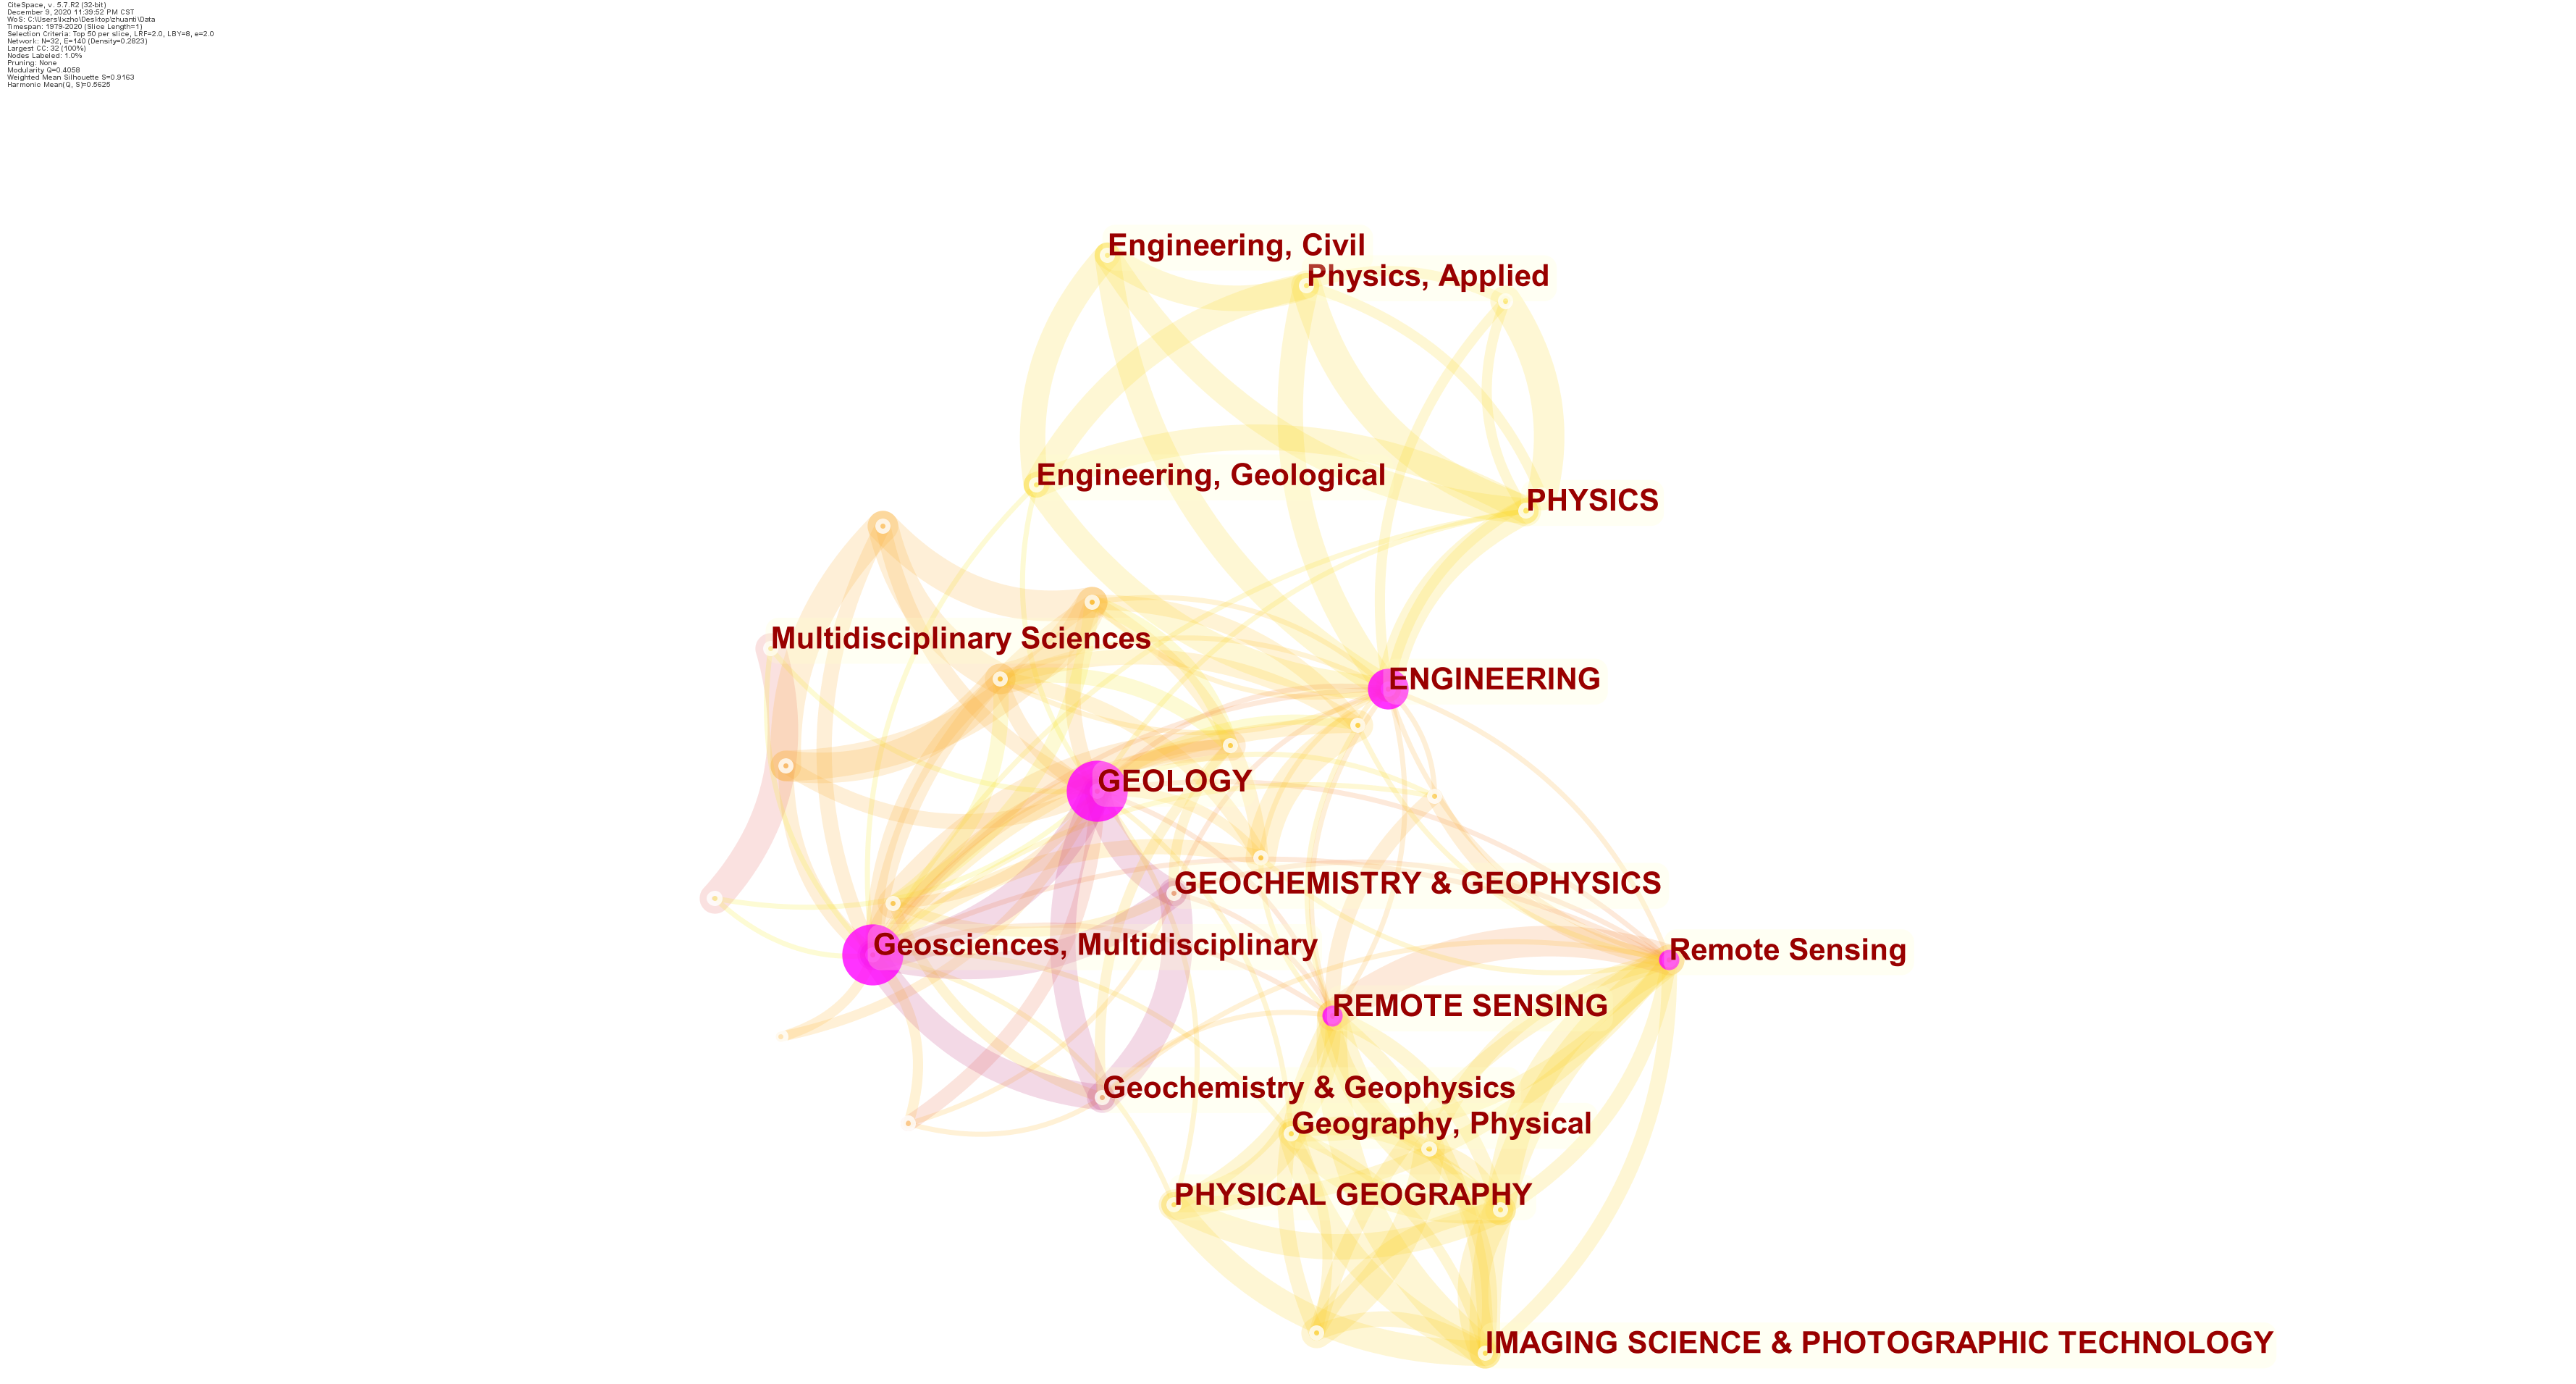
\includegraphics[scale=0.1]{./pic/category.png}\\
  \caption{Category}\label{fig_okada}
\end{figure}
\end{frame}

\begin{frame}
\frametitle{\textcolor{blue}{CiteSpace:}Keywords}
\begin{figure}
  \centering
  % Requires \usepackage{graphicx}
  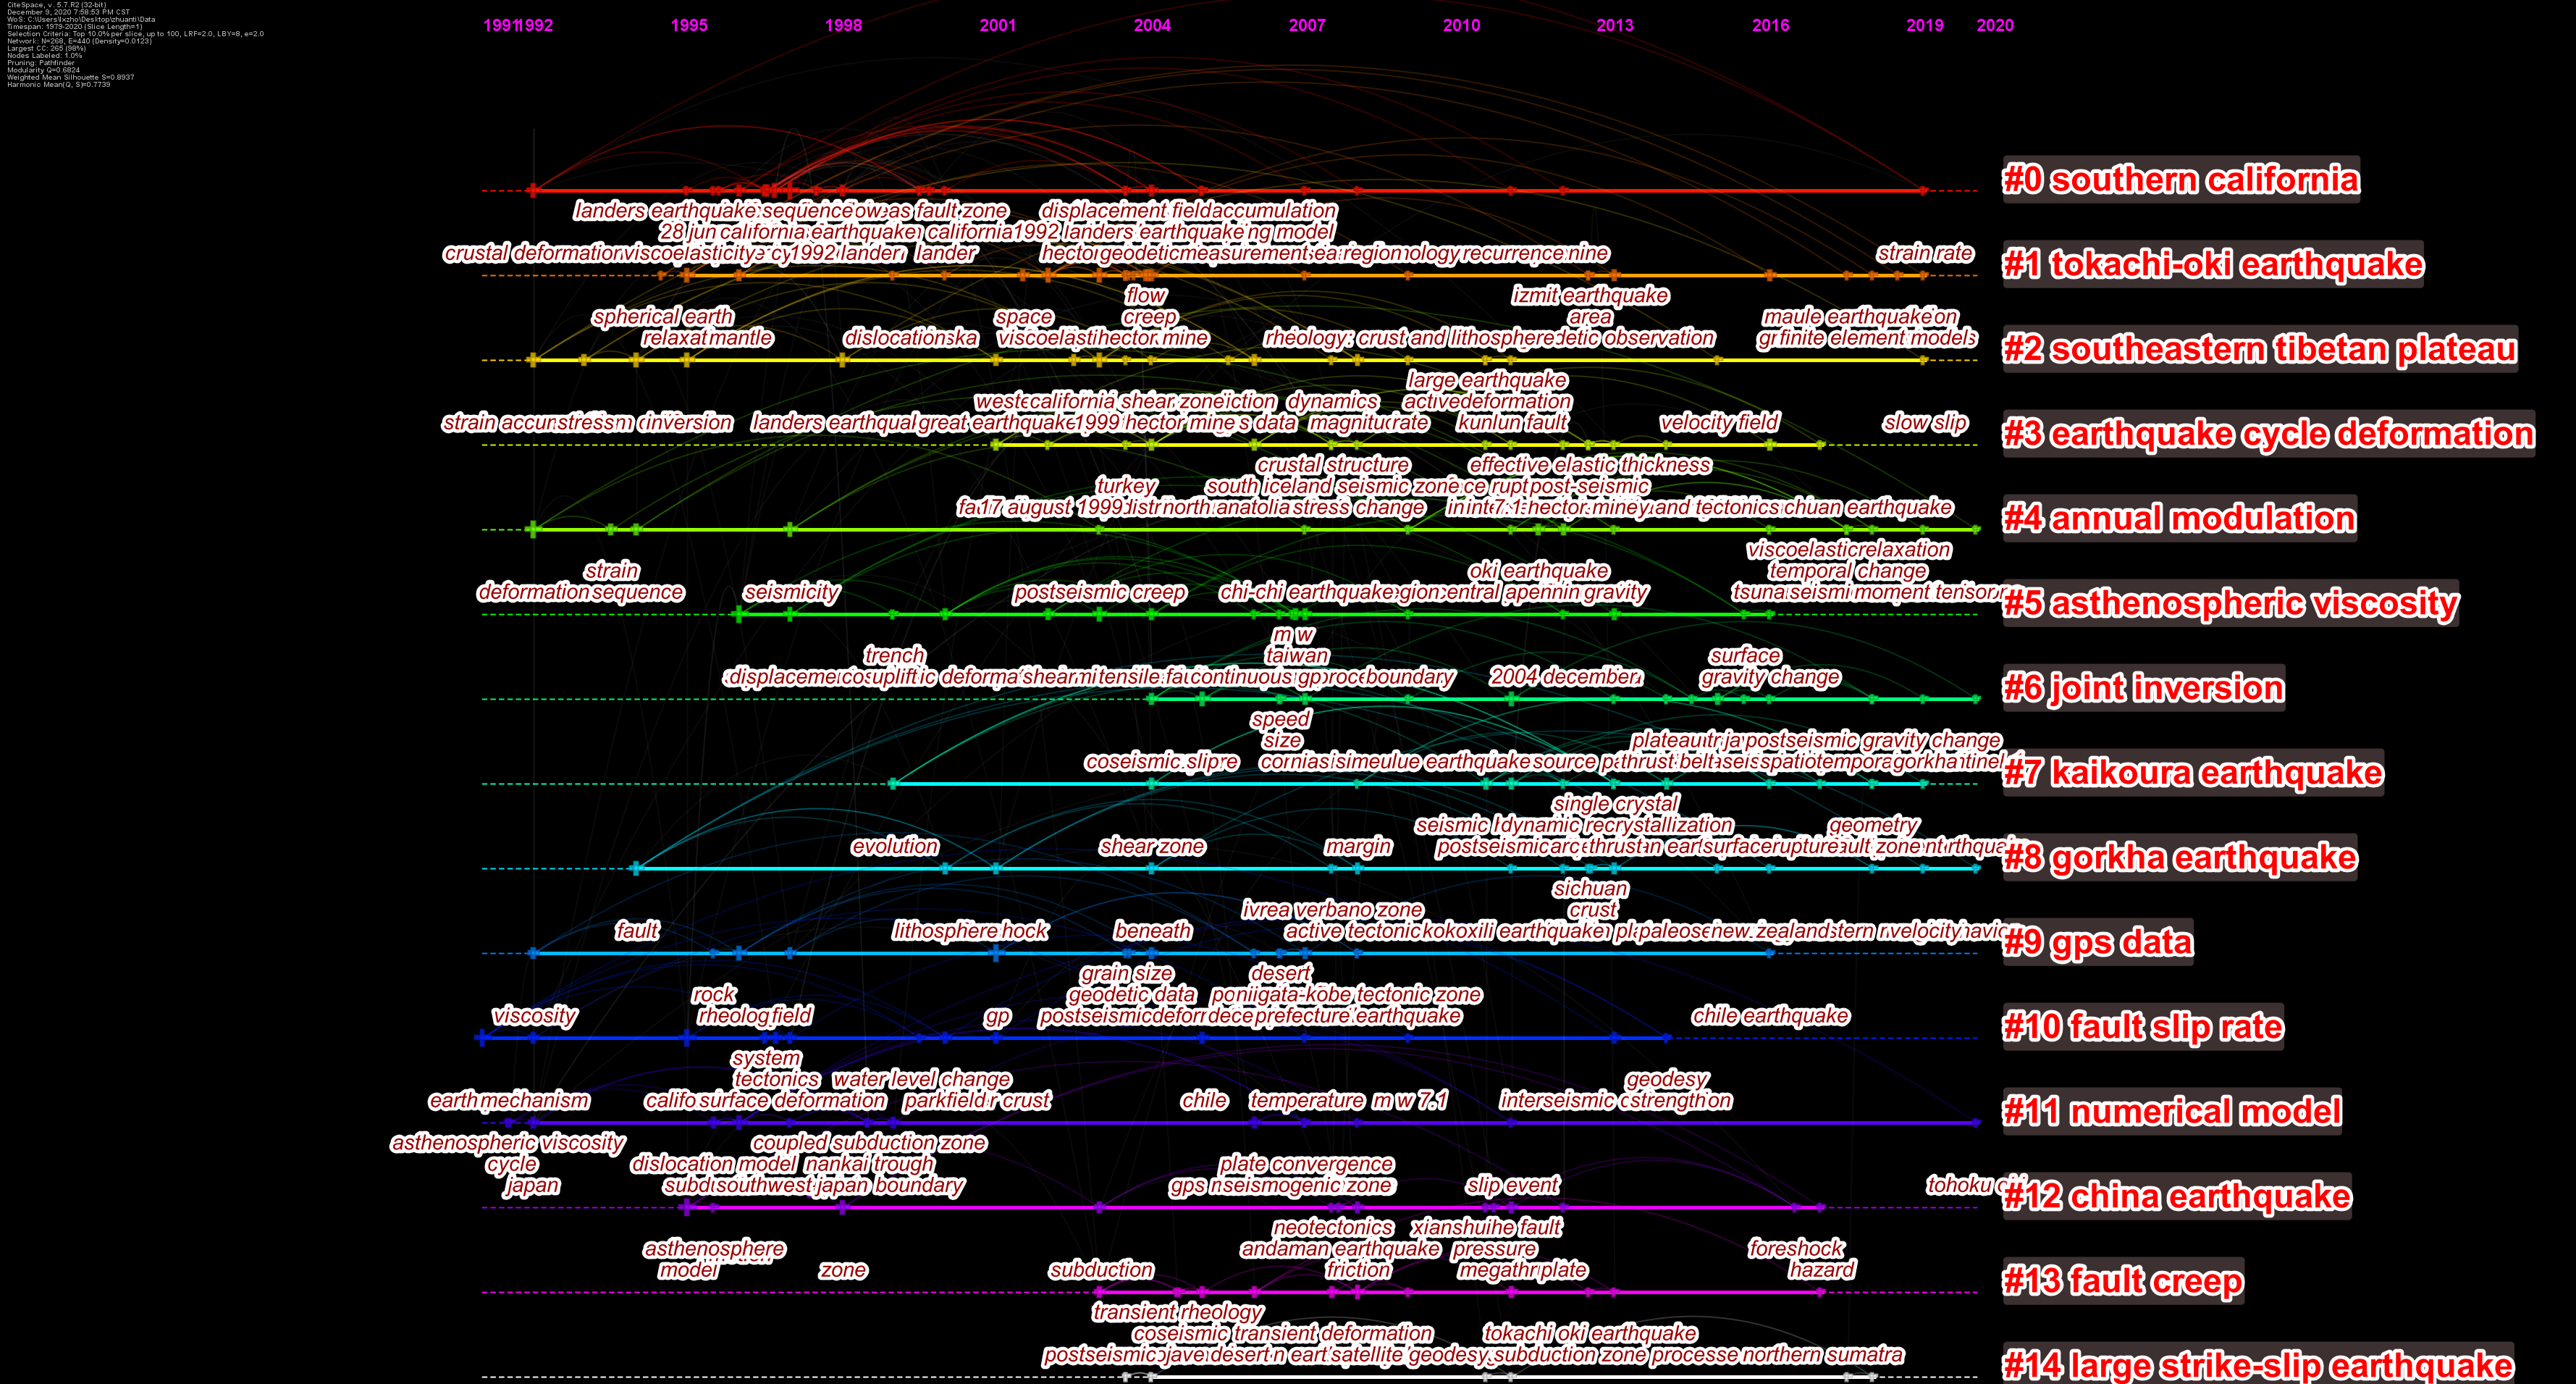
\includegraphics[scale=0.1]{./pic/keywords.png}\\
  \caption{Category}\label{fig_okada}
\end{figure}
\end{frame}

\begin{frame}
\frametitle{\textcolor{blue}{CiteSpace:}Authors}
\begin{figure}
  \centering
  % Requires \usepackage{graphicx}
  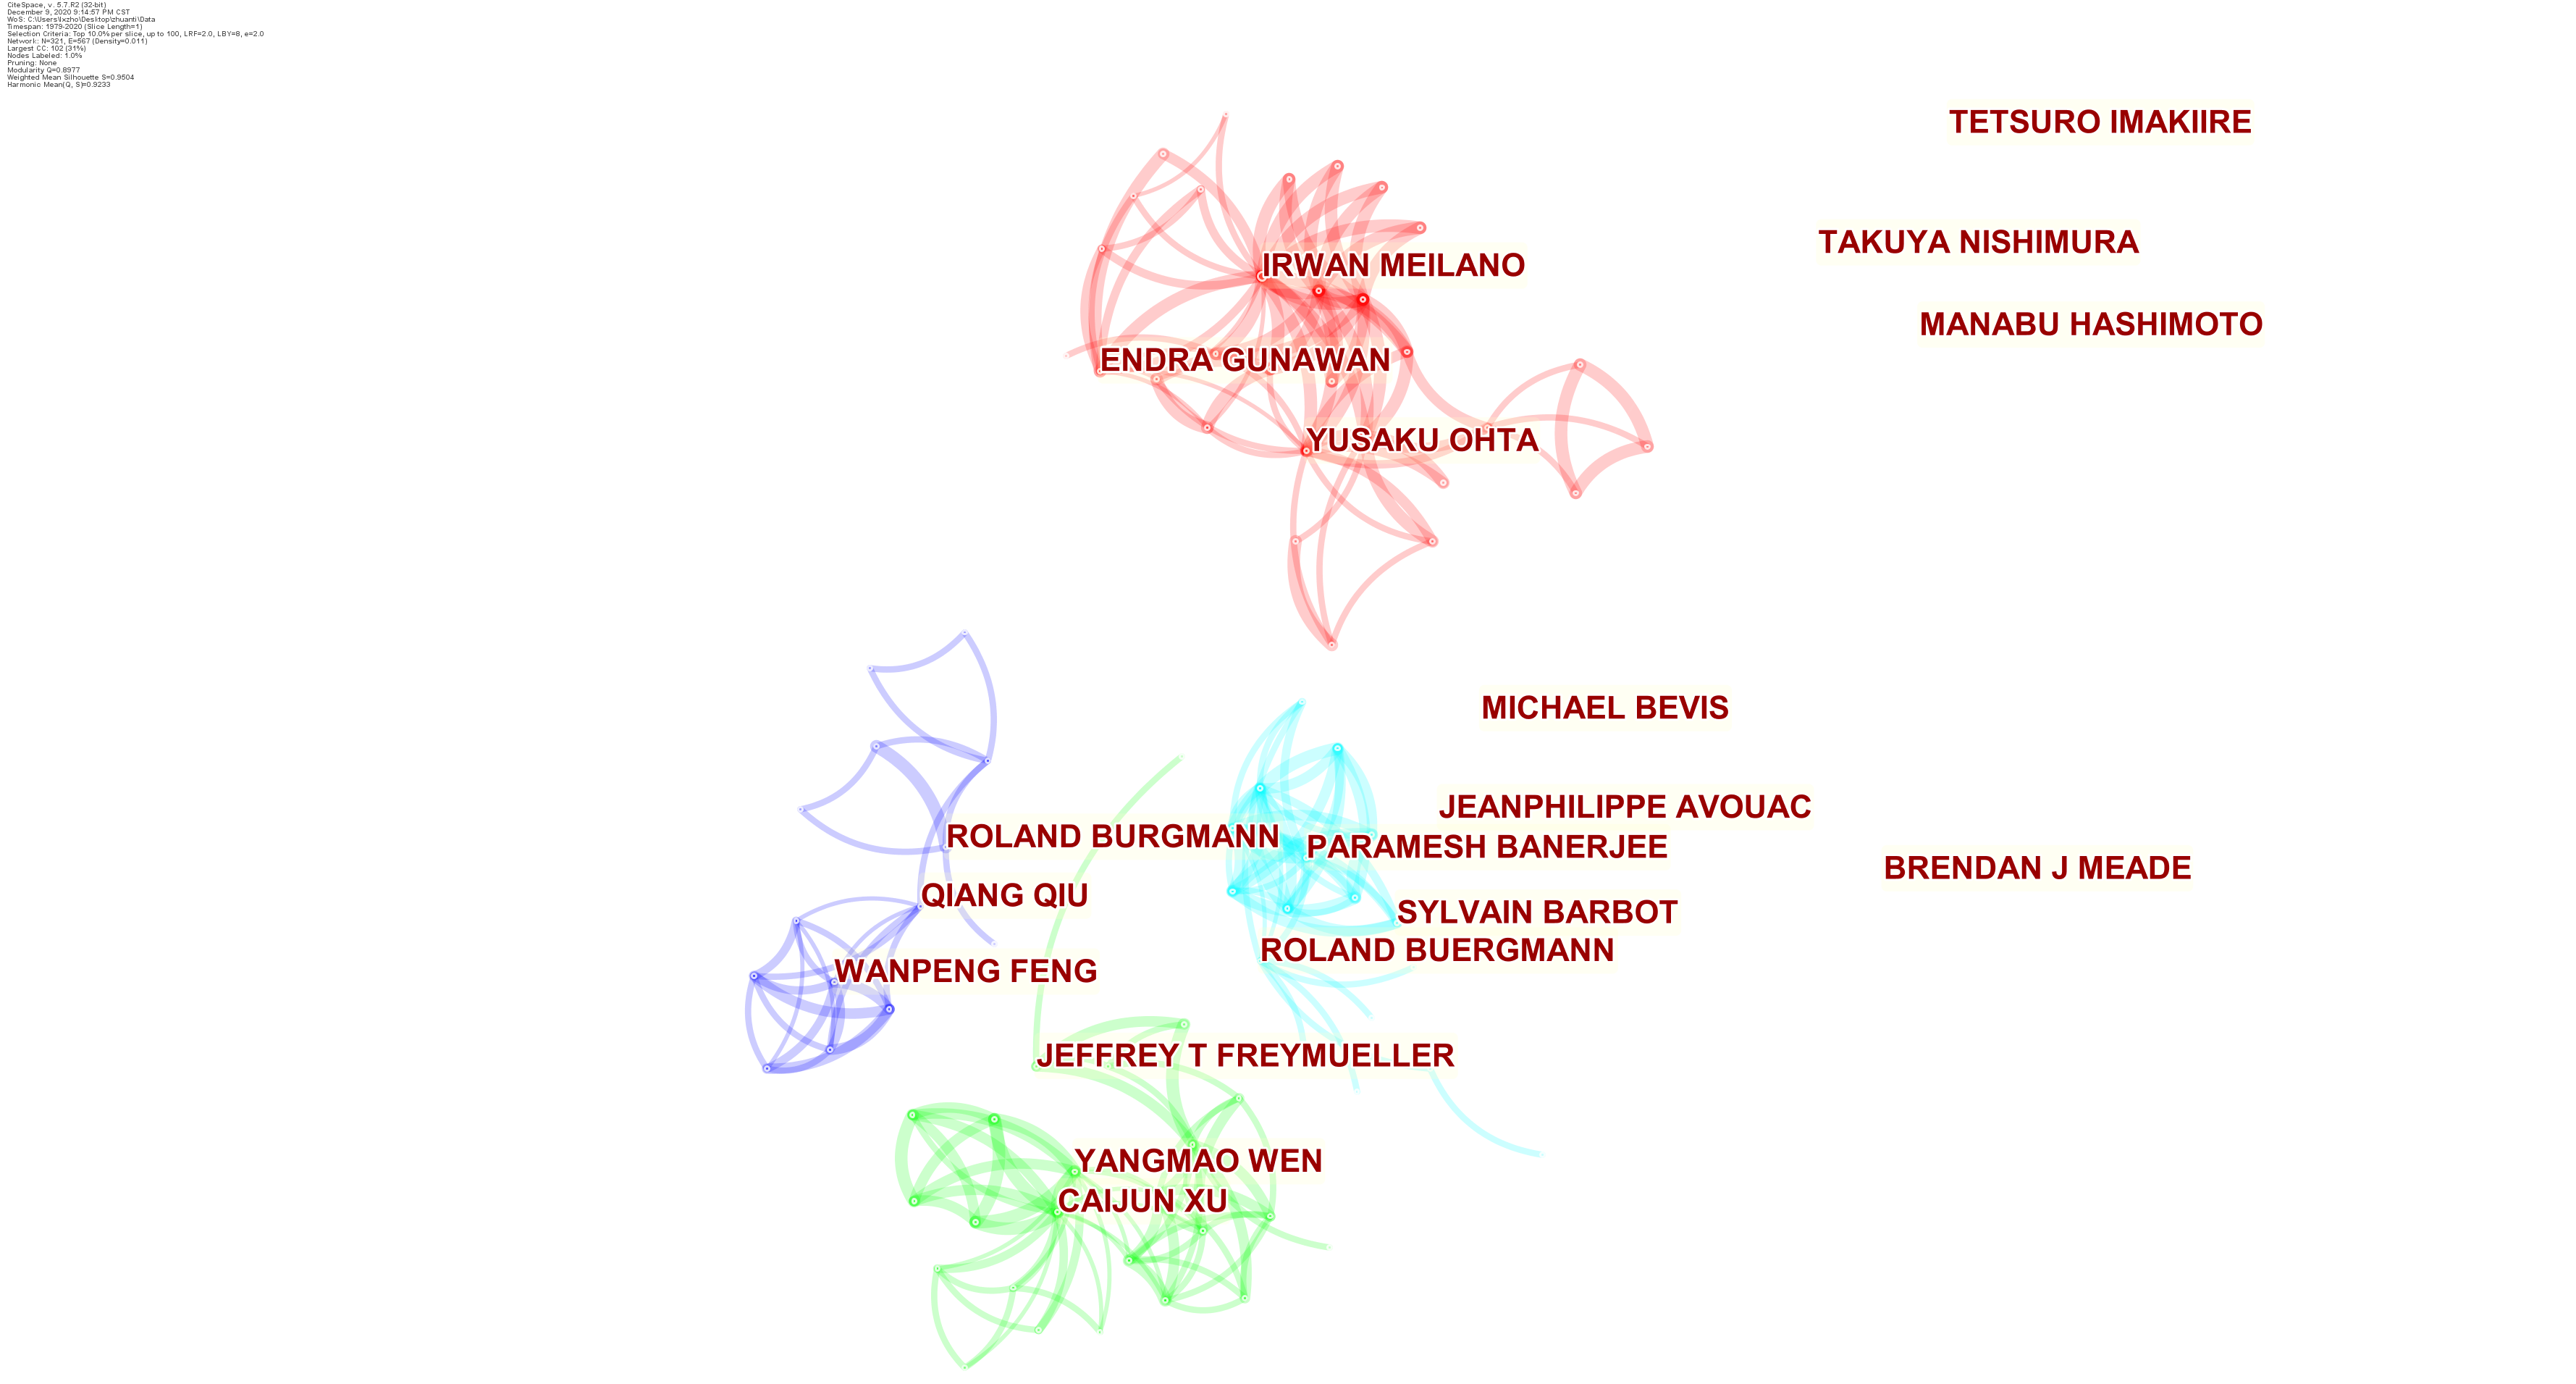
\includegraphics[scale=0.1]{./pic/author.png}\\
  \caption{Authors}\label{fig_okada}
\end{figure}
\end{frame}

\begin{frame}
\frametitle{\textcolor{blue}{CiteSpace:}References}
\begin{figure}
  \centering
  % Requires \usepackage{graphicx}
  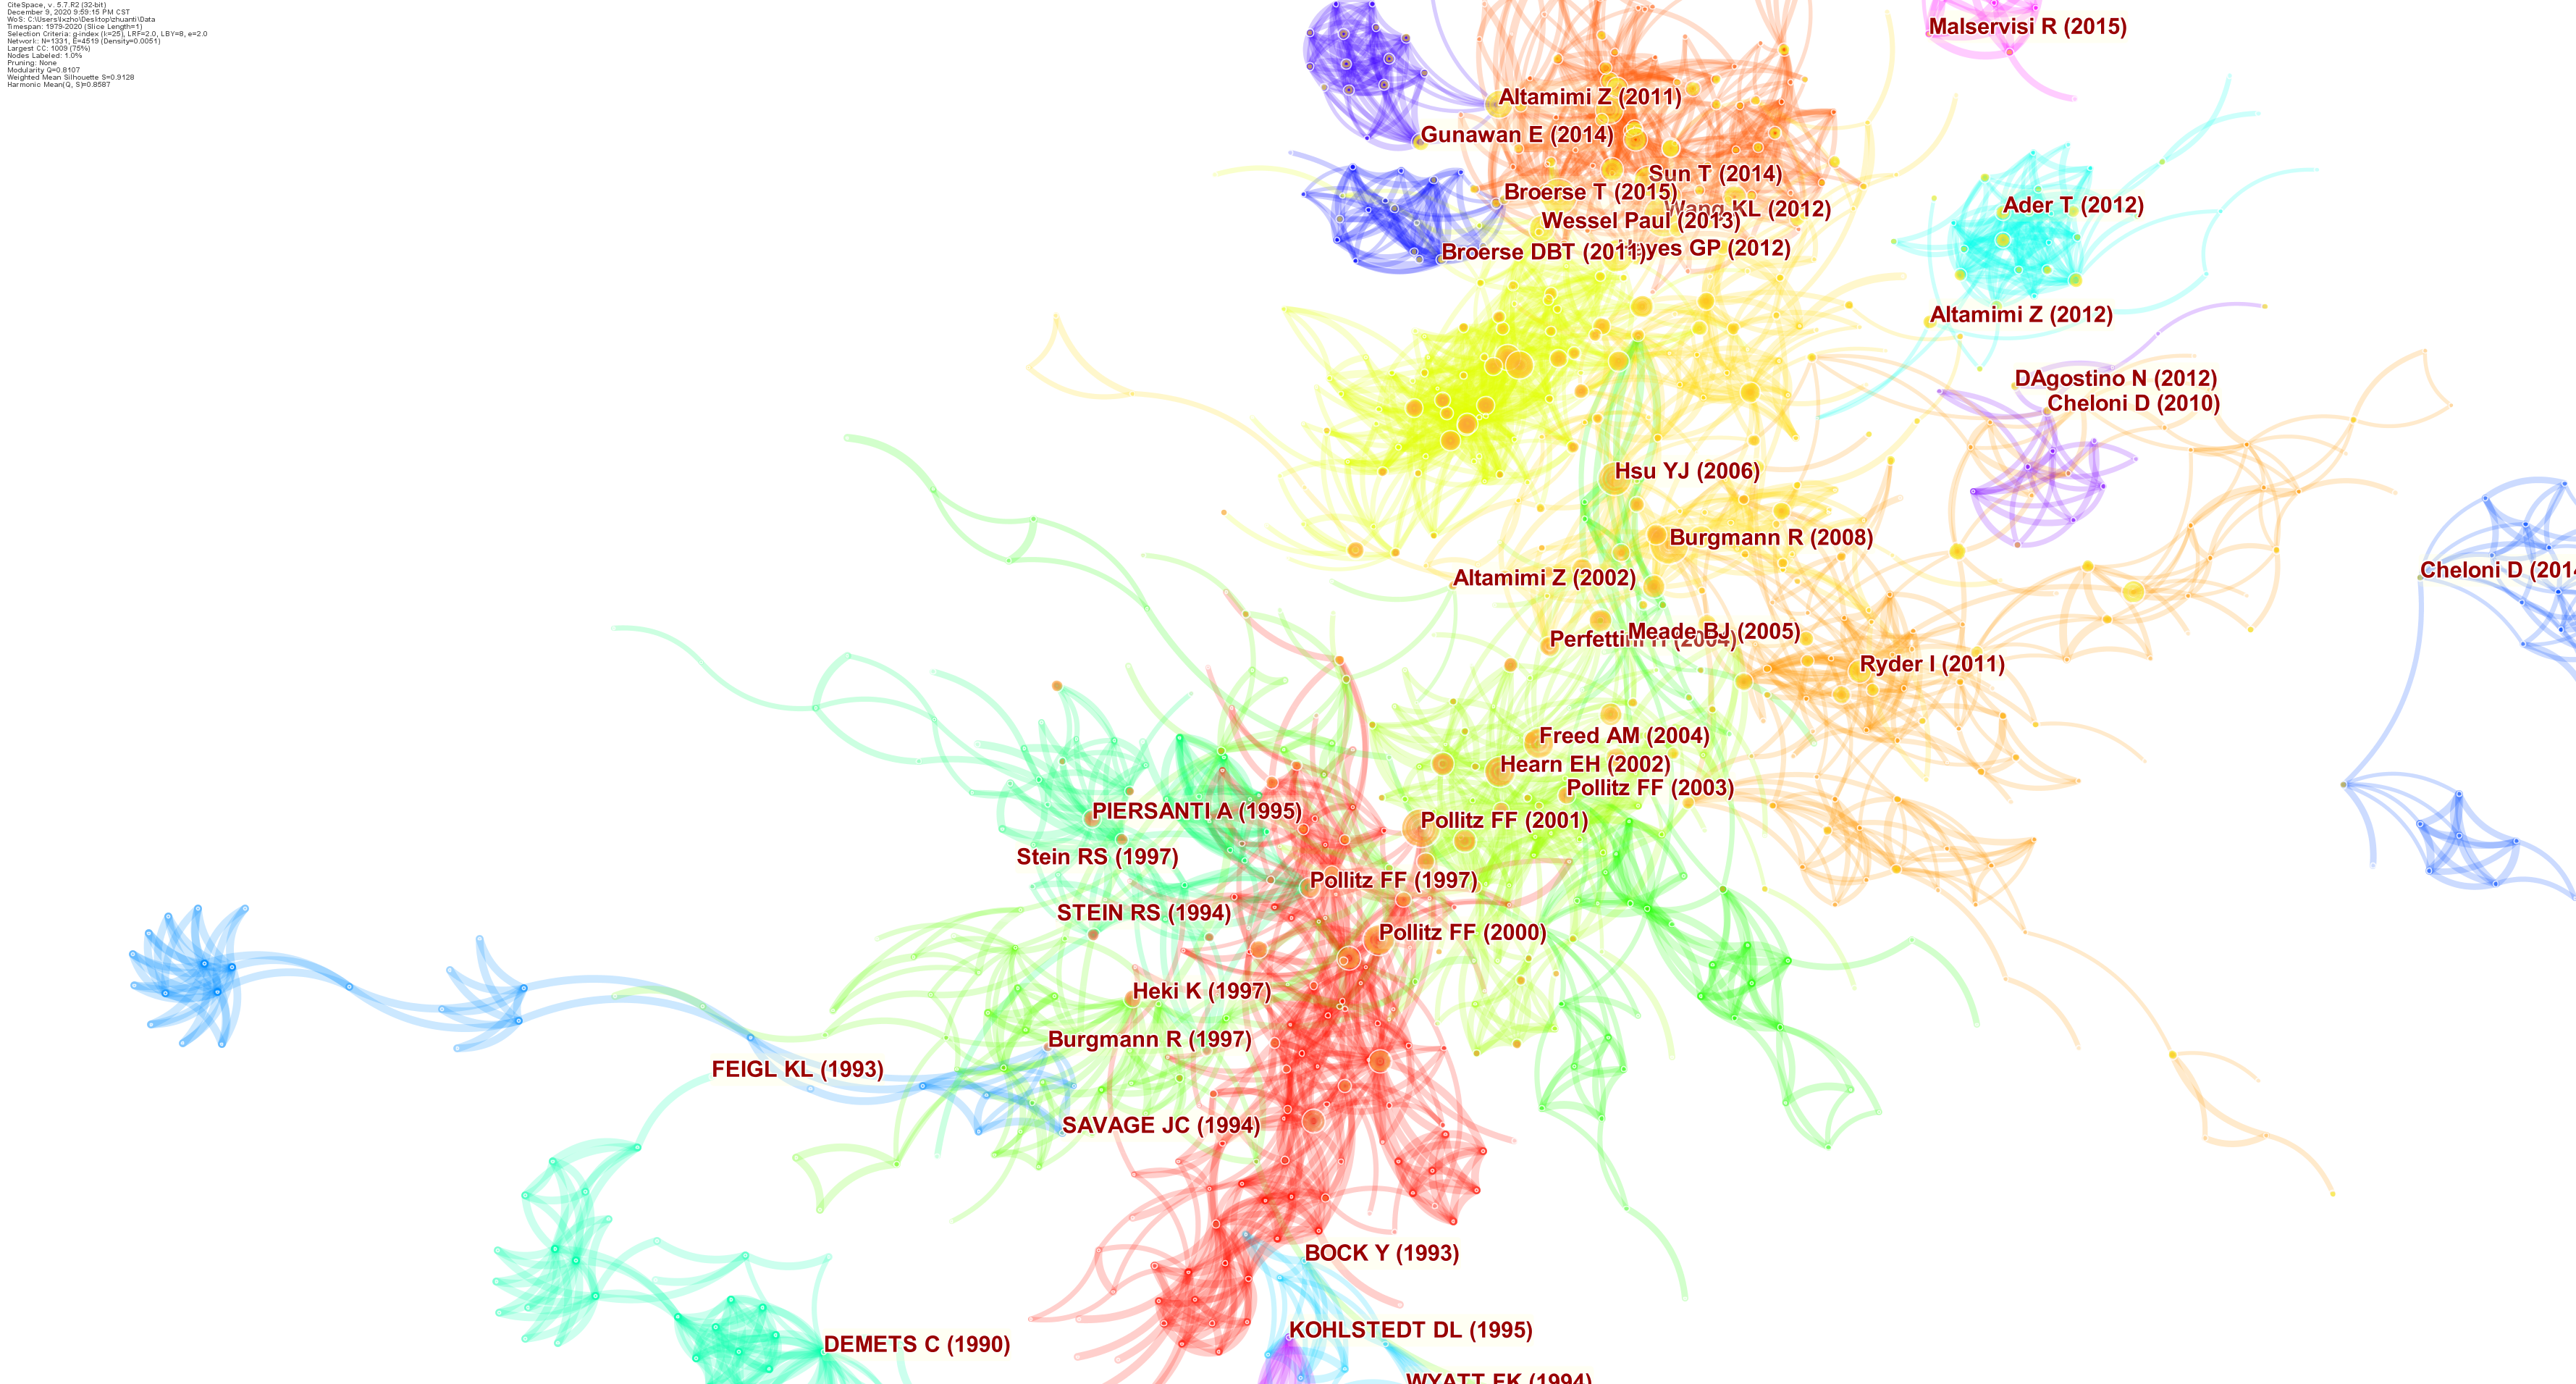
\includegraphics[scale=0.1]{./pic/reference.png}\\
  \caption{Authors}\label{fig_okada}
\end{figure}
\end{frame}

\section{Concepts}
%-----------------------------------------------------
\begin{frame}
\frametitle{Earthquake Cycle}

\begin{columns}[c] % The "c" option specifies centered vertical alignment while the "t" option is used for top vertical alignment

\column{.45\textwidth} % Left column and width
The \textbf{earthquake cycle} is a theoretical framework used by earth scientists to describe the \textcolor{red}{repeating process} of tectonic \textcolor{red}{stress accumulation} between earthquakes and \textcolor{red}{stress release} during earthquake (\textcolor{blue}{Reid 1910; Boulton,2017}).

\column{.5\textwidth} % Right column and width
\begin{figure}
  \centering
  % Requires \usepackage{graphicx}
  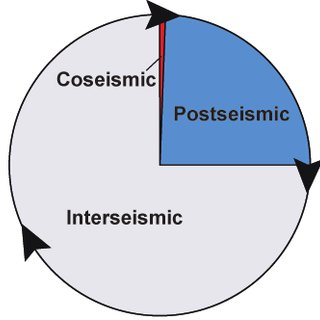
\includegraphics[scale=0.45]{./pic/earthquake_cycle.jpg}\\
  \caption{Schematic figure of the earthquake cycle}\label{fig_okada}
\end{figure}

\end{columns}

\end{frame}

\begin{frame}
\frametitle{Earthquake Cycle}

\begin{columns}[c] % The "c" option specifies centered vertical alignment while the "t" option is used for top vertical alignment

\column{.45\textwidth} % Left column and width
The \textbf{earthquake cycle} is a theoretical framework used by earth scientists to describe the \textcolor{red}{repeating process} of tectonic \textcolor{red}{stress accumulation} between earthquakes and \textcolor{red}{stress release} during earthquake (\textcolor{blue}{Reid 1910; Boulton,2017}).

\column{.5\textwidth} % Right column and width
\begin{figure}
  \centering
  % Requires \usepackage{graphicx}
  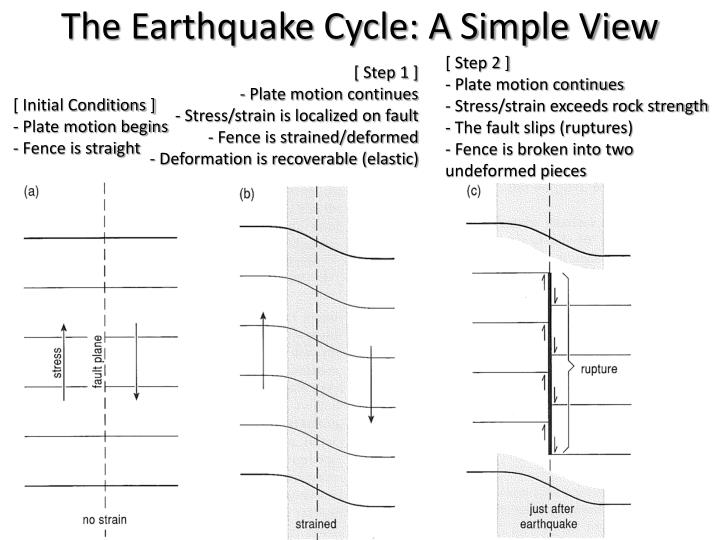
\includegraphics[scale=0.25]{./pic/earthquake_cycle_simple.jpg}\\
  \caption{A simple view of the earthquake cycle}\label{fig_okada}
\end{figure}

\end{columns}

\end{frame}

\begin{frame}
\frametitle{Postseismic Deformation}
Immediately after the occurrence of the earthquake, the mechanism of stress release due to viscous flow in the ductile part of the Earth’s crust starts to operate, leading to \textbf{post-seismic deformation}.

The delayed deformation of the lithosphere caused by stress relaxation in the mantle or in the low viscosity layers of the crust is called \textbf{post-seismic deformation} (\textcolor{blue}{R. Sabadini \& B. Vermeersen, 2004}).
\end{frame}

\begin{frame}
\frametitle{Viscoelasticity}

\textcolor{blue}{黏弹性(Viscoelasticity)}:在外加载荷作用下,应变落后于应力的性质。

\textcolor{blue}{麦克斯韦模型(Maxwell model)}:。一种用以描述固体物质黏弹性质由一个弹簧和一个阻尼器串联组成的简化的理论模型。麦克斯韦体对施加的力的短时间响应像弹性固体,而长时间响应则像黏滞流体。

\textcolor{blue}{开尔文-沃伊特模型(Kelvin-Voight model)}:一种用以描述固体物质的黏弹性质,由一个弹簧和一个阻尼器并联组成的简化的理论模型。

\textcolor{blue}{标准线性固体(standard linear solid)}:性质介于弹性与黏滞性的非完全弹性体,其本构方程可以表示为应力、应力的一阶导数与应变、应变的一阶导数呈线性关系的、既有弹性响应又有黏性响应的介质。


\end{frame}


\begin{frame}
\frametitle{Viscoelasticity}


\begin{figure}
  \centering
  % Requires \usepackage{graphicx}
  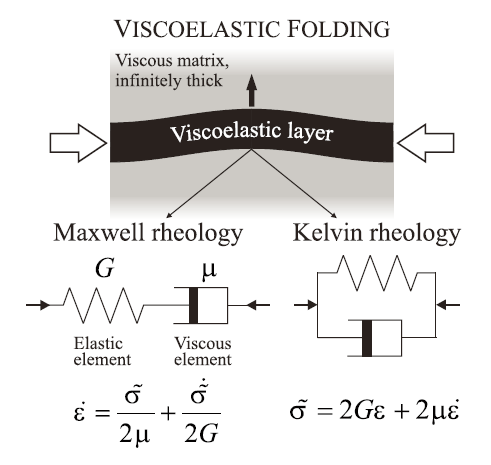
\includegraphics[scale=0.35]{./pic/viscoelastic.png}\\
  \caption{Sketch of viscoelastic folding and presentation of the
two simplest viscoelastic rheologies: the Maxwell and the Kelvin
rheology. In a Maxwell model strains are additive whereas in a
Kelvin model stresses are additive. The equations are given for
deviatoric stresses.(\textcolor{blue}{S.M. Schmalholz et al., 2001})}\label{fig_okada}
\end{figure}



\end{frame}

\begin{frame}
\frametitle{Viscoelasticity}

\begin{columns}[c] % The "c" option specifies centered vertical alignment while the "t" option is used for top vertical alignment

\column{.45\textwidth} % Left column and width
\begin{figure}
  \centering
  % Requires \usepackage{graphicx}
  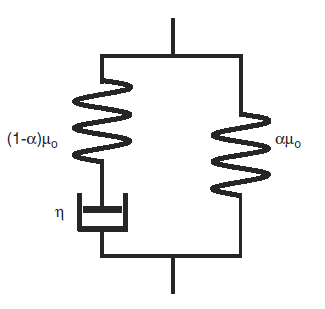
\includegraphics[scale=0.5]{./pic/sls_model.png}\\
  \caption{Model of SLS rheology(\textcolor{blue}{R. Wang et al., 2006})}\label{fig_okada}
\end{figure}

\column{.5\textwidth} % Right column and width
\begin{figure}
  \centering
  % Requires \usepackage{graphicx}
  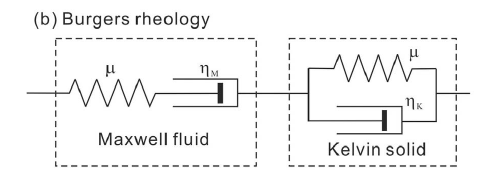
\includegraphics[scale=0.5]{./pic/Burgers.png}\\
  \caption{Cartoon illustration of the Burgers material consisting of the Maxwell fluid in series with the Kelvin solid.(\textcolor{blue}{Yan Hu et al., 2012})}\label{fig_okada}
\end{figure}

\end{columns}

\end{frame}

\begin{frame}
\frametitle{Afterslip}
\textcolor{blue}{Afterslip}又称“后滑动事件(post-seismic slip event)”。在一次大的构造地震(突然的同震滑动)后,断层的位移通过蠕滑增加,产生与主震相当的滑动量的现象。余滑可持续数年,小部分系由余震引起的,但大部分余滑的发生不产生地震波。余滑事件通常遵从大森定律(Omori's law)。

\textcolor{blue}{大森定律 Omori’s law}:又称“大森关系式(Omori's relation)”“双曲线定律(hyperbolic law)”。日本大森房吉(F. Omori)于1894 年得到的余震频次随时间呈反比衰减的定律。
\end{frame}

\begin{frame}
\frametitle{Rate-and-state friction}
At steady-state, both state evolution laws reduce $\theta$ to Dc/V, so that the steady-state coefficient of friction can be simply expressed as (\textcolor{blue}{M.P.A van den Ende et al., 2018}):

$\mu_{ss}(V)=\mu^{*}+(a-b)ln(\frac{V}{V^*})$
\\

\tiny{
\begin{enumerate}
  \item The parameter (a−b) now describes the velocity-dependence of $\mu$ at steady-state, with \textbf{positive values} (i.e. a>b) resulting in \textbf{velocity strengthening}, and \textcolor{red}{negative values} resulting in \textcolor{red}{velocity-weakening} behaviour.
  \item It has been demonstrated by Ruina (1983) that a material characterised by a negative (a−b) is prone to frictional instabilities, i.e. stick-slip behaviour, and thus it is assumed that \textbf{seismogenic fault segments exhibit a negative (a−b)}.
  \item \textbf{Typical values for (a−b)} reported by experimental studies lie in the range of $\pm 10^{-3}-10^{-2}$.
\end{enumerate}
}
\end{frame}

\begin{frame}
\frametitle{Poroelastic Rebound}
After the earthquake, fluids will migrate from high-pressure areas to low pressure
areas resulting in time-dependent surface deformation associated with\textbf{ poroelastic rebound} (\textcolor{blue}{Peltzer et al., 1996, 1998; Yan Hu et al., 2014}).
\end{frame}

\section{Why}
\begin{frame}
\frametitle{Significance}
\begin{enumerate}
  \item Understanding the mechanical strength (\textbf{rheology}) of the lithosphere and the processes that govern postseismic stress transfer is central to our \textbf{understanding of the earthquake cycle and seismic hazards} (\textcolor{blue}{Freed et al., 2006}).
  \item Inferences from postseismic studies provide insights into some of the most \textbf{basic properties of the lithosphere}, such as the \textcolor{blue}{constitutive properties} and \textcolor{blue}{extent of faulting}, \textcolor{blue}{the permeability of the crust} and \textcolor{blue}{influence of fluid flow}, the \textcolor{blue}{depth extent of the elastic portion} of the crust, and the \textcolor{blue}{relative viscoelastic strength} of the lower crust and upper mantle (\textcolor{blue}{Freed et al., 2006}).
  \item Important part of the \textbf{ITRF2014} (\textcolor{blue}{Altamimi et al., 2016}).
\end{enumerate}

\end{frame}
\section{Problems-How-Prospects}
\begin{frame}
\frametitle{Problems}

\begin{enumerate}
  \item List some of the \textbf{software} related to the postseismic deformation?
  \item How to \textbf{extract} the 'pure' postseismic deformation?
  \item How to get the \textbf{viscosity} or \textbf{frictional parameters}?
\end{enumerate}

\end{frame}

\begin{frame}
\frametitle{Software}
\begin{figure}
  \centering
  % Requires \usepackage{graphicx}
  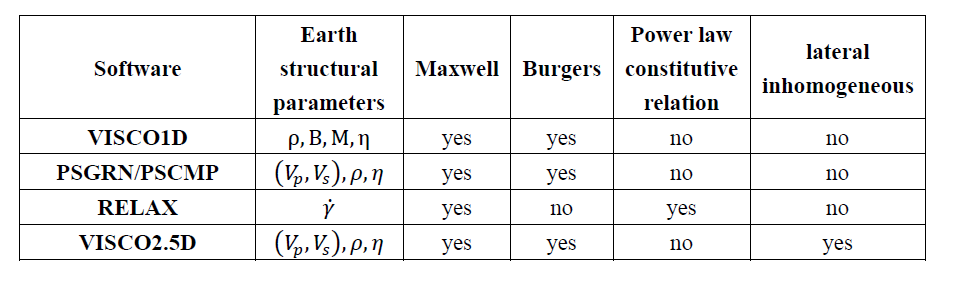
\includegraphics[scale=0.4]{./pic/soft11.png}\\
  \caption{粘弹性松弛软件比较(\textcolor{blue}{赵斌, 2017})}\label{fig_okada}
\end{figure}

\end{frame}

\begin{frame}
\frametitle{Software}
\begin{figure}
  \centering
  % Requires \usepackage{graphicx}
  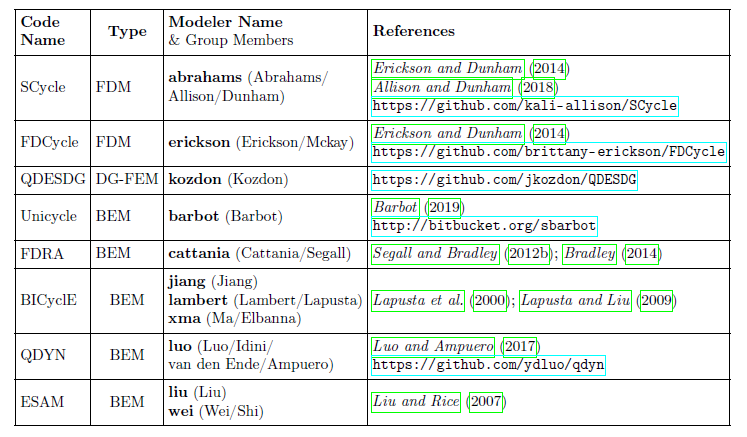
\includegraphics[scale=0.5]{./pic/soft2.png}\\
  \caption{Codes for simulating sequences of earthquake and aseismic slip (SEAS)(\textcolor{blue}{Erickson et al.,2019})}\label{fig_okada}
\end{figure}

\end{frame}


\begin{frame}
\frametitle{\textbf{Extract} the 'pure' postseismic deformation}
The raw time series obtained from GPS observations usually contain various signals, such as: \textbf{offsets} related to earthquake or antenna/receiver changes; \textbf{secular velocities} due to plate motion or fault locking; \textbf{seasonal variations} which mainly come from hy-drological loading (\textcolor{blue}{Zhen Tian et al., 2020}).


\end{frame}

\begin{frame}
\frametitle{\textbf{Extract} the 'pure' postseismic deformation}
\small{
\begin{itemize}
  \item \textbf{Preprocessing} the data, such as eliminating outliers, repairing nonseismic offsets and correcting coseismic offsets.
  \item \textbf{Interpolating} the interseismic 3-D velocities of the stations installed after the mainshock. The computer code VISR (velocity interpolation for strain rate) developed by Shen et al. (2015) is applied to interpolate the inter-seismic velocities of those stations without preearthquake observations.
  \item Determining the \textbf{logarithmic relaxation time} after removing longterm
trends and seasonal items.
  \item \textbf{Improving} the signal-to-noise ratio of postseismic displacements
using the PCA algorithm. (\textcolor{blue}{Z.S. Jiang et al., 2018})
\end{itemize}

}

\end{frame}

\begin{frame}
\frametitle{\textbf{Extract} the 'pure' postseismic deformation}
\small{
$y(t)_{preseismic}=A+Bt+Csin(2\pi t)+Dcos(2\pi t)+Esin(4\pi t)+Fcos(4\pi t)+H(t)$
$y(t)_{postseismic}=\alpha ln(1+\frac{t}{\tau})+\beta sin(2\pi t)+\gamma cos(2\pi t)+H(t)+\delta$
}

(\textcolor{blue}{Ingleby et al., 2020})
\end{frame}

\begin{frame}
\frametitle{\textbf{Extract} the 'pure' postseismic deformation}

\begin{columns}[c] % The "c" option specifies centered vertical alignment while the "t" option is used for top vertical alignment

\column{.45\textwidth} % Left column and width
\begin{figure}
  \centering
  % Requires \usepackage{graphicx}
  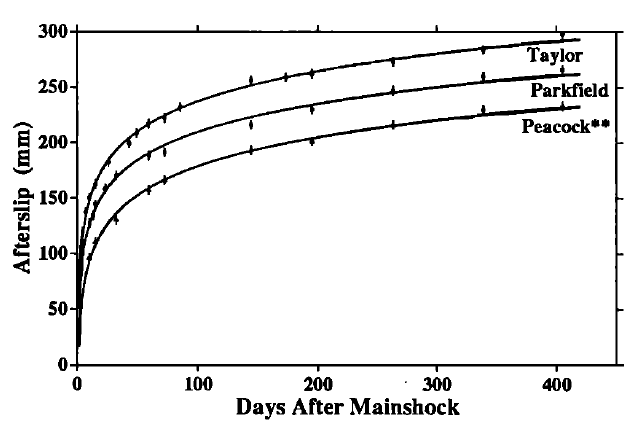
\includegraphics[scale=0.3]{./pic/Marone1991.png}\\
  \caption{“\textbf{Transient after slip creep}” behavior [Marone et al., 1991;
Perfettini and Avouac, 2004; Savage et al., 2005] tending to follow a \textbf{logarithmic} function.}\label{fig_okada}
\end{figure}

\column{.5\textwidth} % Right column and width
\begin{figure}
  \centering
  % Requires \usepackage{graphicx}
  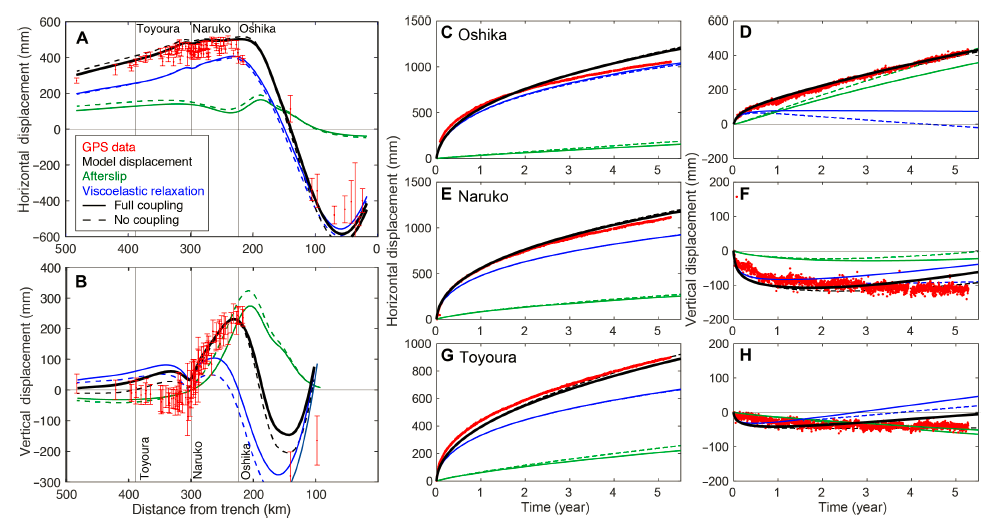
\includegraphics[scale=0.2]{./pic/muto2019.png}\\
  \caption{“\textbf{Viscoelastic relaxation}” type [Savage and Prescott, 1978; Pollitz, 1997] that is better described by an \textbf{exponential} decay (Muto et al., 2019).}\label{fig_okada}
\end{figure}

\end{columns}

\end{frame}

\begin{frame}
\frametitle{Viscosity or frictional parameters}
\begin{enumerate}
  \item Trial and error method
  \item Grid search method
  \item ABIC
  \item Adjoint method
\end{enumerate}
\end{frame}

\begin{frame}
\frametitle{Viscosity or frictional parameters}
\begin{figure}
  \centering
  % Requires \usepackage{graphicx}
  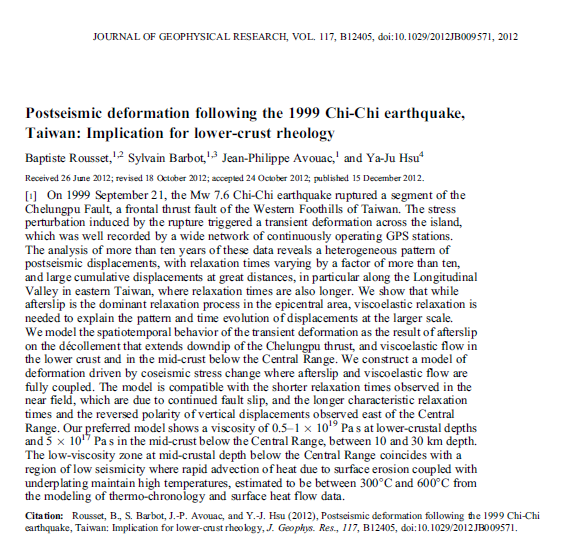
\includegraphics[scale=0.4]{./pic/trial.png}\\
  \caption{Trial and error method}\label{fig_okada}
\end{figure}

\end{frame}

\begin{frame}
\frametitle{Viscosity or frictional parameters}
\begin{figure}
  \centering
  % Requires \usepackage{graphicx}
  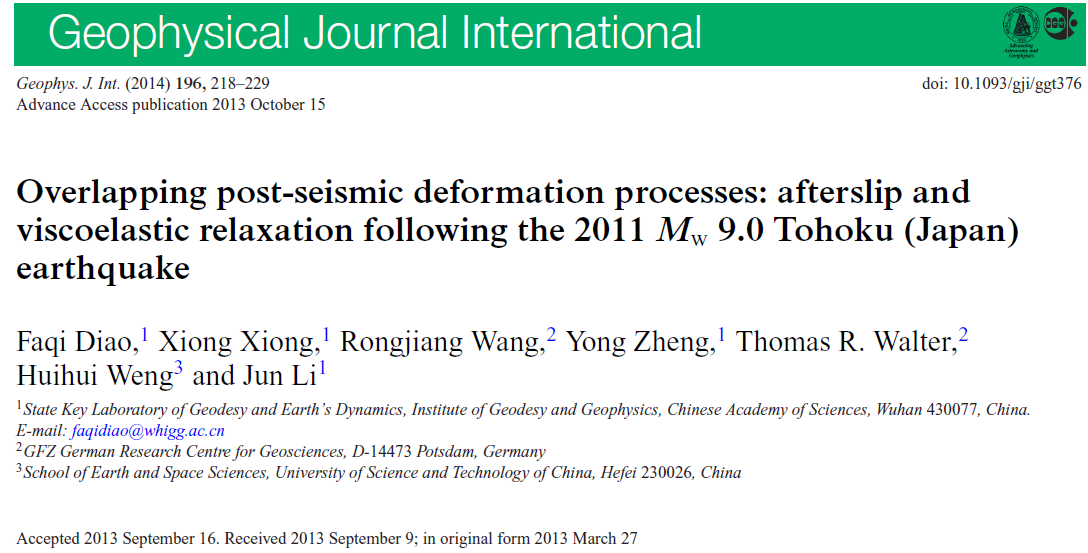
\includegraphics[scale=0.4]{./pic/grid.png}\\
  \caption{Grid search method}\label{fig_okada}
\end{figure}

\end{frame}

\begin{frame}
\frametitle{Viscosity or frictional parameters}

\begin{columns}[c] % The "c" option specifies centered vertical alignment while the "t" option is used for top vertical alignment

\column{.45\textwidth} % Left column and width
\begin{figure}
  \centering
  % Requires \usepackage{graphicx}
  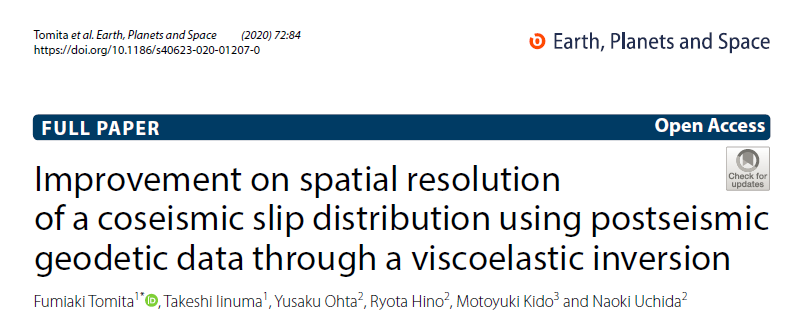
\includegraphics[scale=0.3]{./pic/abic.png}\\
  \caption{ABIC}\label{fig_okada}
\end{figure}

\column{.45\textwidth}
\begin{figure}
  \centering
  % Requires \usepackage{graphicx}
  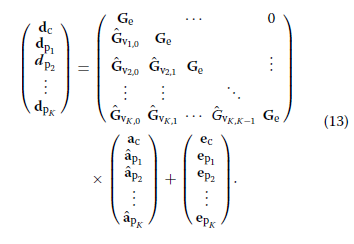
\includegraphics[scale=0.4]{./pic/abic2.png}\\
  \caption{Model}\label{fig_okada}
\end{figure}

\end{columns}

\end{frame}

\begin{frame}
\frametitle{Viscosity or frictional parameters}

\begin{columns}[c] % The "c" option specifies centered vertical alignment while the "t" option is used for top vertical alignment

\column{.45\textwidth} % Left column and width
\begin{figure}
  \centering
  % Requires \usepackage{graphicx}
  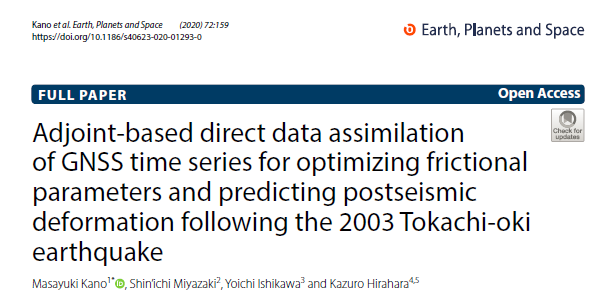
\includegraphics[scale=0.3]{./pic/adjoint1.png}\\
  \caption{Adjoint method}\label{fig_okada}
\end{figure}

\column{.45\textwidth}
\begin{figure}
  \centering
  % Requires \usepackage{graphicx}
  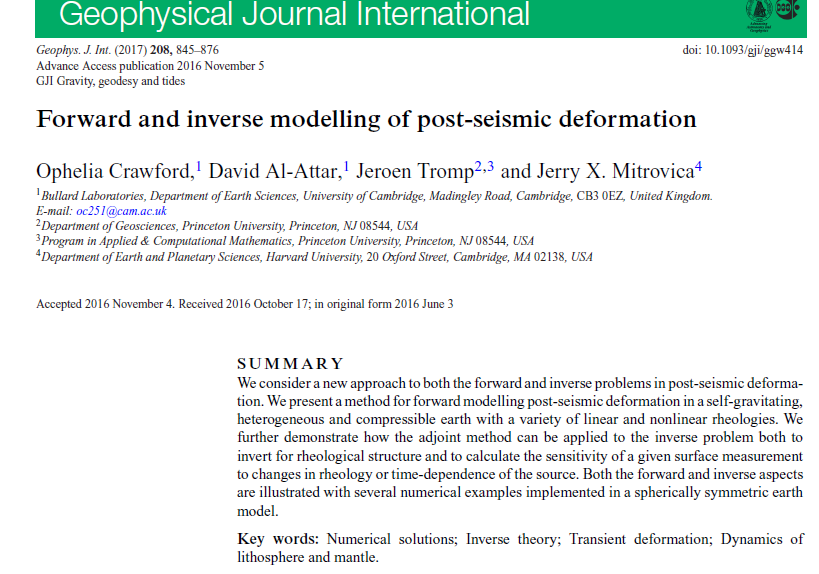
\includegraphics[scale=0.25]{./pic/adjoint2.png}\\
  \caption{Adjoint method}\label{fig_okada}
\end{figure}

\end{columns}

\end{frame}


\section{Conclusion}
\begin{frame}
\begin{enumerate}
  \item Develop \textbf{softwares} that simulate the postseismic deformation
  \item Compare the methods of \textbf{extracting 'pure'} postseismic deformation
  \item Propose \textbf{new methods or ways to invert} for the viscosity and frictional parameters
  \item Analyse the postseismic deformation to find \textbf{new phenomenon or knowledge}.
\end{enumerate}
\end{frame}

\begin{frame}
\frametitle{Problems}

\begin{enumerate}
  \item Could we use the postseismic deformation to \textbf{constraint the fault geometry}?
  \item How to \textbf{seperate} the effect of various postseismic mechanisms?
  \item What is the \textbf{relationship} among the coseismic slip distribution, afterslip distribution, and occurrence of aftershocks?
  \item When do viscoelastic relaxation and afterslip \textbf{begin} and \textbf{how long} will they last in near- and far-field?
  \item Is the friction properties of the fault \textbf{stationary}?
\end{enumerate}

\end{frame}

\begin{frame}
\begin{figure}
  \centering
  % Requires \usepackage{graphicx}
  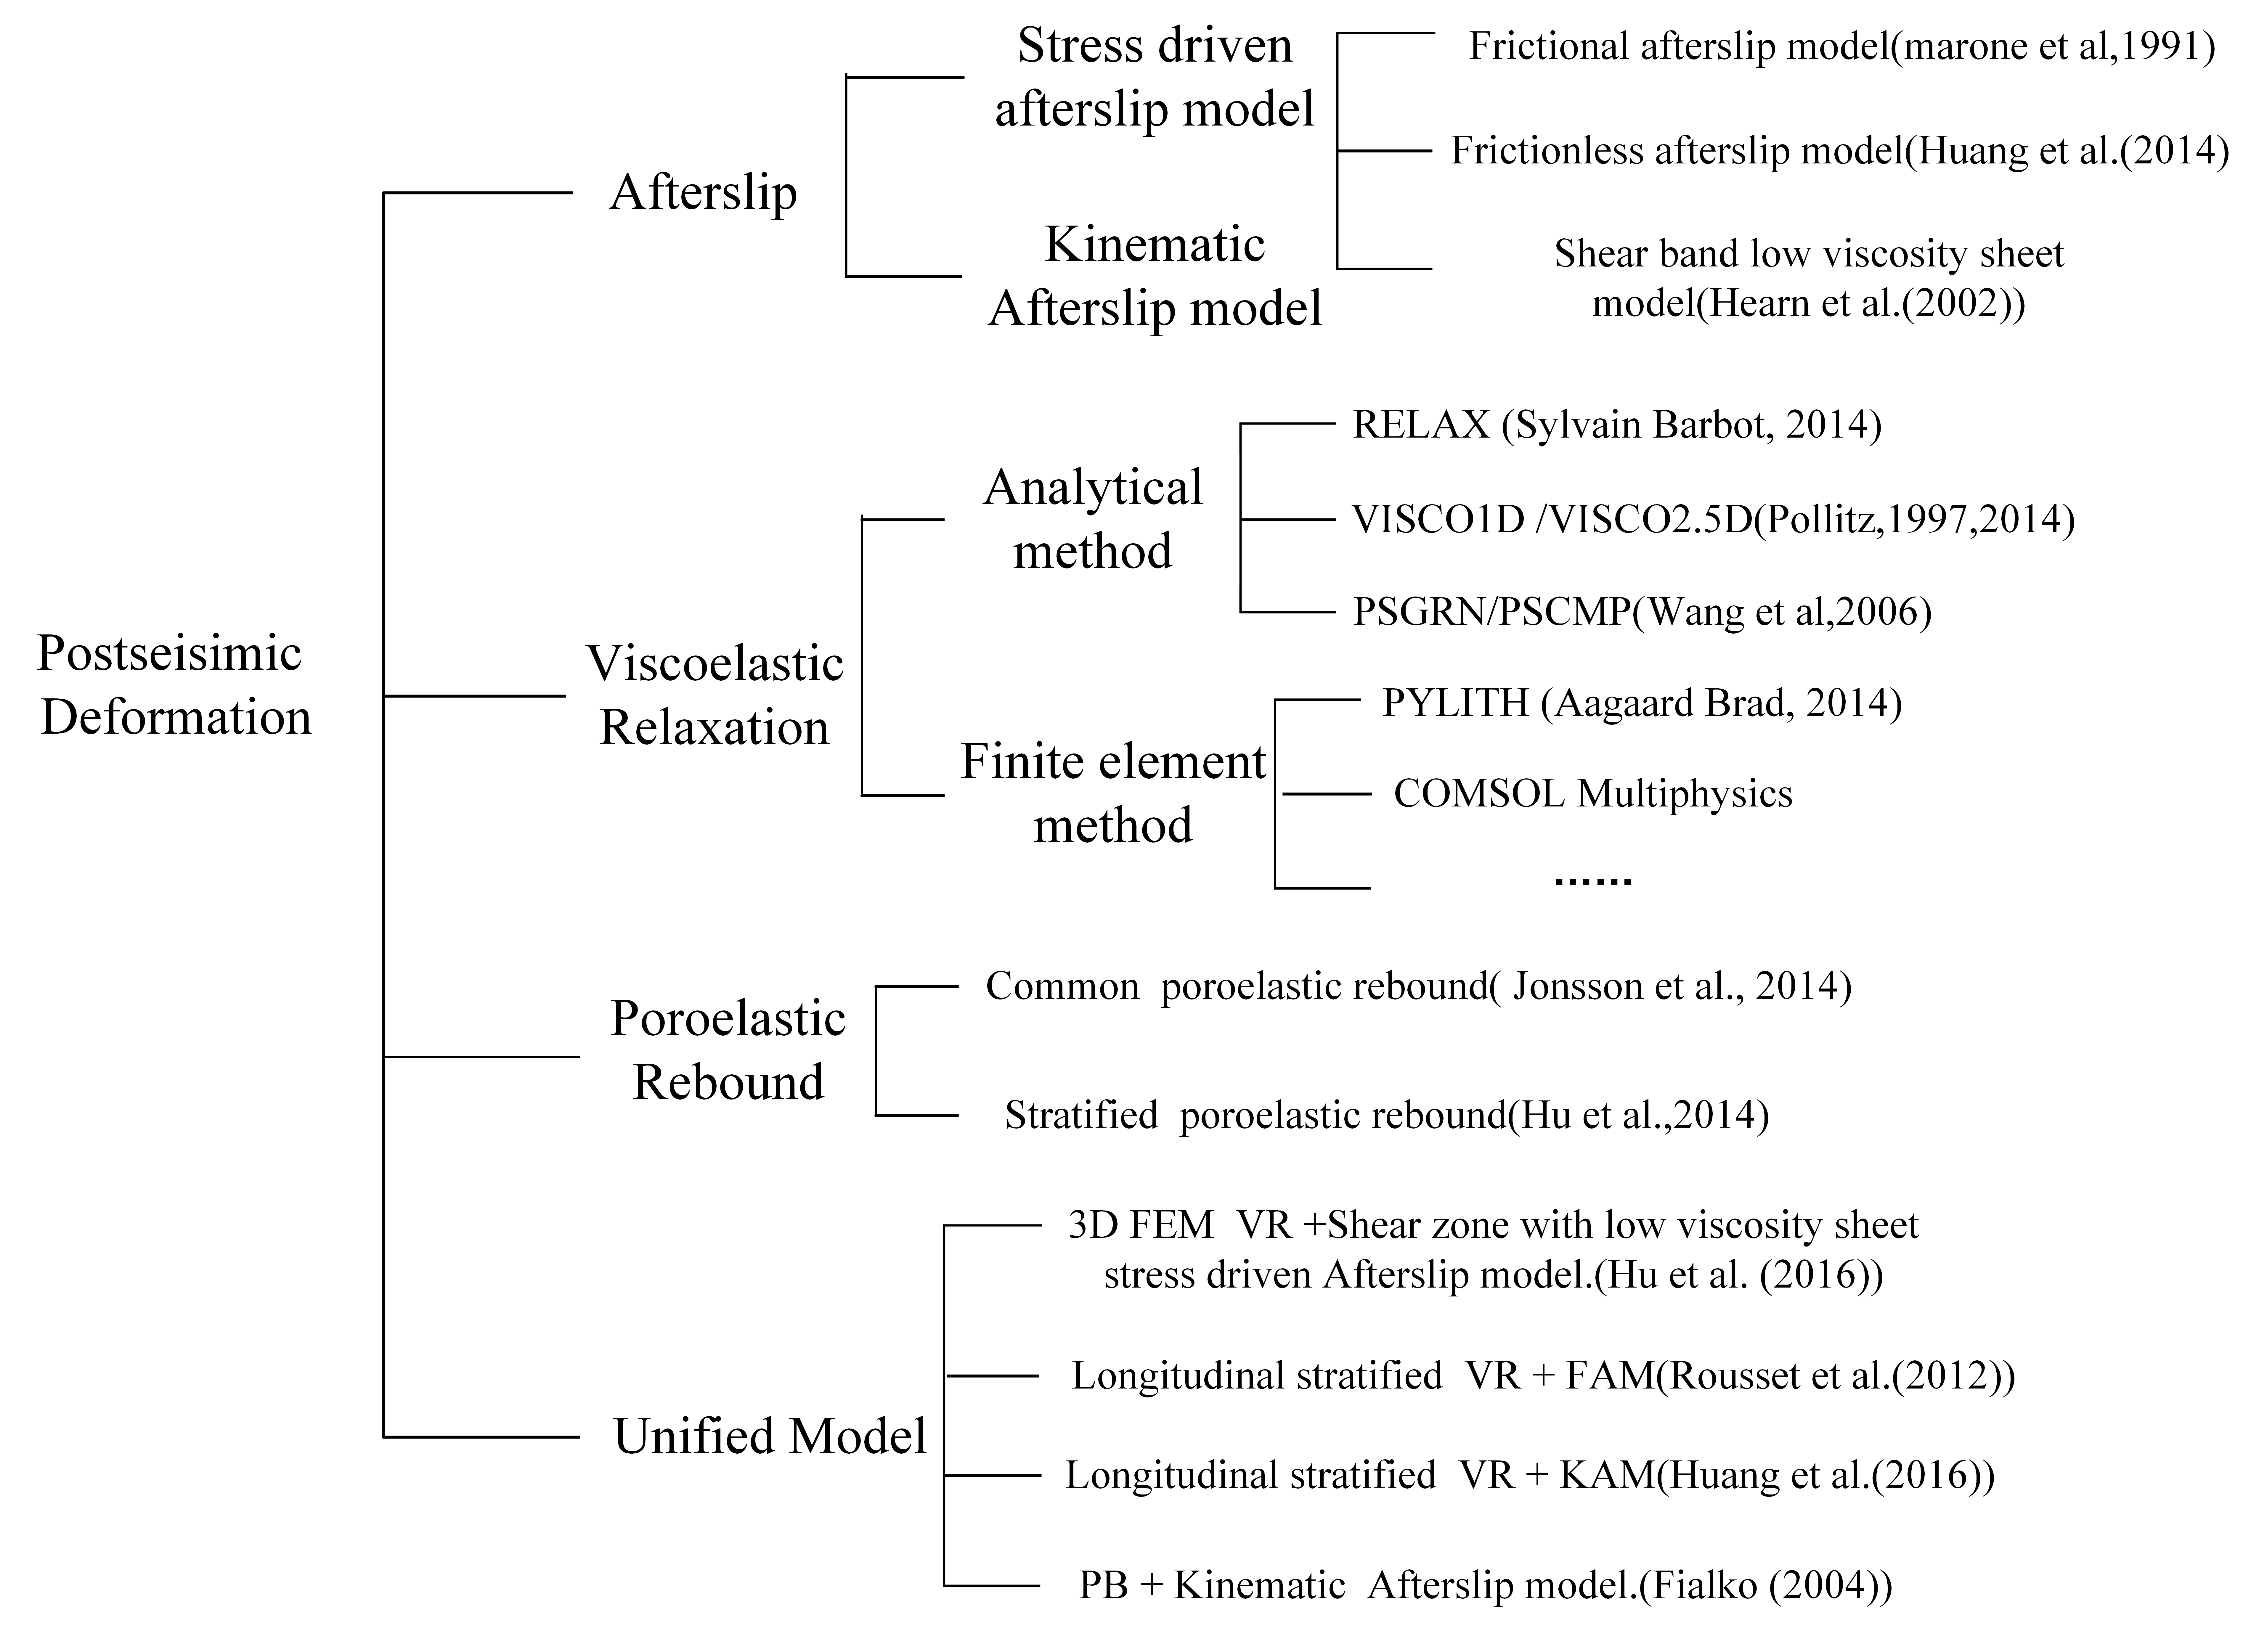
\includegraphics[scale=0.42]{./pic/diagram.jpg}\\
  \caption{}\label{fig_okada}
\end{figure}
\end{frame}


\begin{comment}


%------------------------------------------------
\begin{frame}
\frametitle{Bullet Points}
\begin{itemize}
\item Lorem ipsum dolor sit amet, consectetur adipiscing elit
\item Aliquam blandit faucibus nisi, sit amet dapibus enim tempus eu
\item Nulla commodo, erat quis gravida posuere, elit lacus lobortis est, quis porttitor odio mauris at libero
\item Nam cursus est eget velit posuere pellentesque
\item Vestibulum faucibus velit a augue condimentum quis convallis nulla gravida
\end{itemize}
\end{frame}

%------------------------------------------------
\begin{frame}
\frametitle{Blocks of Highlighted Text}
\begin{block}{Block 1}
Lorem ipsum dolor sit amet, consectetur adipiscing elit. Integer lectus nisl, ultricies in feugiat rutrum, porttitor sit amet augue. Aliquam ut tortor mauris. Sed volutpat ante purus, quis accumsan dolor.
\end{block}

\begin{block}{Block 2}
Pellentesque sed tellus purus. Class aptent taciti sociosqu ad litora torquent per conubia nostra, per inceptos himenaeos. Vestibulum quis magna at risus dictum tempor eu vitae velit.
\end{block}

\begin{block}{Block 3}
Suspendisse tincidunt sagittis gravida. Curabitur condimentum, enim sed venenatis rutrum, ipsum neque consectetur orci, sed blandit justo nisi ac lacus.
\end{block}
\end{frame}

%------------------------------------------------
\begin{frame}
\frametitle{Multiple Columns}
\begin{columns}[c] % The "c" option specifies centered vertical alignment while the "t" option is used for top vertical alignment

\column{.45\textwidth} % Left column and width
\textbf{Heading}
\begin{enumerate}
\item Statement
\item Explanation
\item Example
\end{enumerate}

\column{.5\textwidth} % Right column and width
Lorem ipsum dolor sit amet, consectetur adipiscing elit. Integer lectus nisl, ultricies in feugiat rutrum, porttitor sit amet augue. Aliquam ut tortor mauris. Sed volutpat ante purus, quis accumsan dolor.

\end{columns}
\end{frame}

%------------------------------------------------
\begin{frame}
\frametitle{Table}
\begin{table}
\begin{tabular}{l l l}
\toprule
\textbf{Treatments} & \textbf{Response 1} & \textbf{Response 2}\\
\midrule
Treatment 1 & 0.0003262 & 0.562 \\
Treatment 2 & 0.0015681 & 0.910 \\
Treatment 3 & 0.0009271 & 0.296 \\
\bottomrule
\end{tabular}
\caption{Table caption}
\end{table}
\end{frame}

%------------------------------------------------
\begin{frame}
\frametitle{Theorem}
\begin{theorem}[Mass--energy equivalence]
$E = mc^2$
\end{theorem}
\end{frame}

%------------------------------------------------
\begin{frame}[fragile] % Need to use the fragile option when verbatim is used in the slide
\frametitle{Verbatim}
\begin{example}[Theorem Slide Code]
\begin{verbatim}
\begin{frame}
\frametitle{Theorem}
\begin{theorem}[Mass--energy equivalence]
$E = mc^2$
\end{theorem}
\end{frame}\end{verbatim}
\end{example}
\end{frame}

%------------------------------------------------
\begin{frame}
\frametitle{Figure}
Uncomment the code on this slide to include your own image from the same directory as the template .TeX file.
%\begin{figure}
%\includegraphics[width=0.8\linewidth]{test}
%\end{figure}
\end{frame}

%------------------------------------------------

\begin{frame}[fragile] % Need to use the fragile option when verbatim is used in the slide
\frametitle{Citation}
An example of the \verb|\cite| command to cite within the presentation:\\~

This statement requires citation \cite{p1}.
\end{frame}

%------------------------------------------------

\begin{frame}
\frametitle{References}
\footnotesize{
\begin{thebibliography}{99} % Beamer does not support BibTeX so references must be inserted manually as below
\bibitem[Smith, 2012]{p1} John Smith (2012)
\newblock Title of the publication
\newblock \emph{Journal Name} 12(3), 45 -- 678.
\end{thebibliography}
}
\end{frame}
\end{comment}

\section{}
\begin{frame}
%\Huge{\centerline{谢谢大家}}
%\Huge{\centerline{敬请指导}}
\centerline{\fontsize{50pt}{50pt}{谢谢大家}}
\centerline{\fontsize{50pt}{24pt}{敬请指导}}
\end{frame}

\begin{frame}
\begin{figure}
  \centering
  % Requires \usepackage{graphicx}
  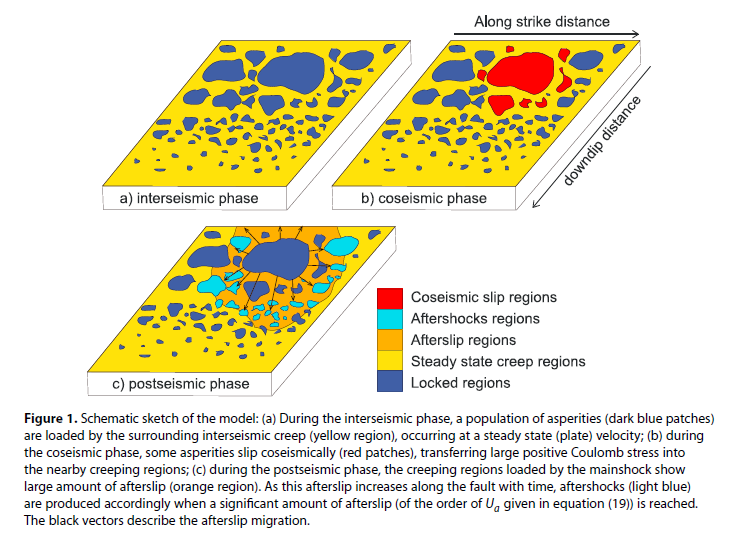
\includegraphics[scale=0.5]{./pic/position.png}\\
  \caption{H. Perfettini et al., 2018. A model of aftershock migration driven by afterslip. GRL.}\label{fig_okada}
\end{figure}
\end{frame}


\begin{frame}

\begin{columns}[c] % The "c" option specifies centered vertical alignment while the "t" option is used for top vertical alignment

\column{.45\textwidth} % Left column and width
\begin{figure}
  \centering
  % Requires \usepackage{graphicx}
  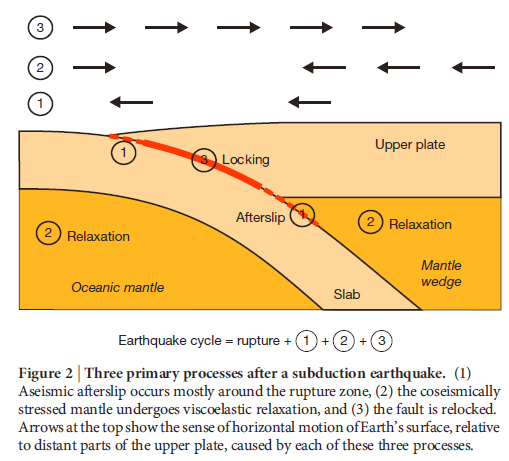
\includegraphics[scale=0.35]{./pic/wangnature.png}\\
  \caption{Kelin Wang et al., 2012. Deformation cycles of subduction earthquakes in a viscoelastic earth. Nature.}\label{fig_okada}
\end{figure}

\column{.45\textwidth}
\begin{figure}
  \centering
  % Requires \usepackage{graphicx}
  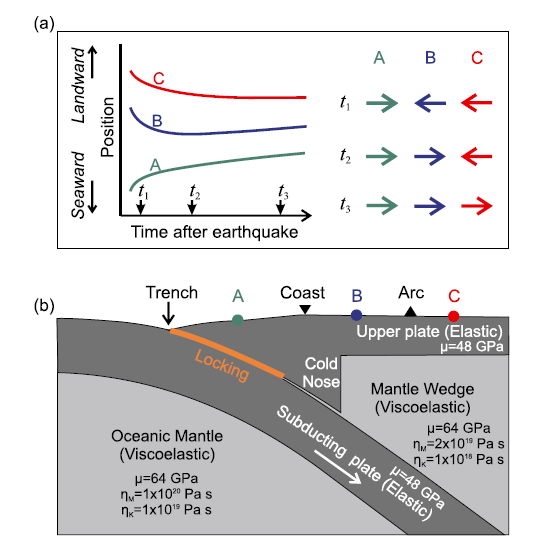
\includegraphics[scale=0.35]{./pic/luo2020.png}\\
  \caption{Haipeng Luo et al., 2020. EPSL}\label{fig_okada}
\end{figure}

\end{columns}

\end{frame}

\begin{frame}
\begin{figure}
  \centering
  % Requires \usepackage{graphicx}
  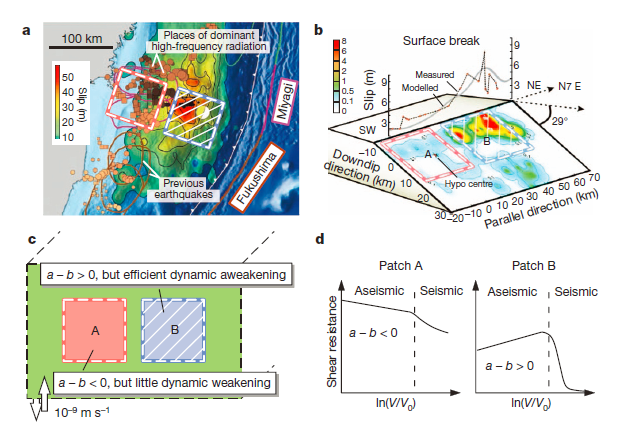
\includegraphics[scale=0.65]{./pic/noda2013.png}\\
  \caption{Noda et al., 2013. Nature.}\label{fig_okada}
\end{figure}
\end{frame}

\end{document}
